% \documentclass[aspectratio=169,notes]{beamer}
\documentclass[aspectratio=169]{beamer}
\usetheme[faculty=phil]{fibeamer}
\usepackage{polyglossia}
\setmainlanguage{english} %% main locale instead of `english`, you
%% can typeset the presentation in either Czech or Slovak,
%% respectively.
\setotherlanguages{russian} %% The additional keys allow
%%
%%   \begin{otherlanguage}{czech}   ... \end{otherlanguage}
%%   \begin{otherlanguage}{slovak}  ... \end{otherlanguage}
%%
%% These macros specify information about the presentation
\title[Introduction to Robotics (In2Ro)]{Introduction to Robotics, Lecture 5} %% that will be typeset on the
\subtitle{Workspace and Singularities 
\\ \ \\ \  } %% title page.
\author{Oleg Bulichev}
%% These additional packages are used within the document:
\usepackage{ragged2e}  % `\justifying` text
\usepackage{booktabs}  % Tables
\usepackage{tabularx}
\usepackage{tikz}      % Diagrams
\usetikzlibrary{calc, shapes, backgrounds, trees, positioning, arrows.meta}
\usetikzlibrary{decorations.pathreplacing,calligraphy,calc,graphs}
\usepackage{amsmath, amssymb}
\usepackage{url}       % `\url`s
\usepackage{listings}  % Code listings
\usepackage{floatrow}
\usepackage{subcaption}
\usepackage{mathtools}
\usepackage{todonotes}
\usepackage{fontspec}
\usepackage{multicol}
\usepackage{pdfpages}
\usepackage{wrapfig}
\usepackage{qrcode}
\usepackage{animate}
\usepackage{booktabs}
\usepackage{multirow}
\usepackage{graphicx}
\usepackage{colortbl}

\graphicspath{{resources/}}
\frenchspacing

\setbeamertemplate{caption}{\raggedright\insertcaption\par}
\usetikzlibrary{graphs}

% \usepackage[backend=biber,style=ieee,autocite=footnote]{biblatex}
% \addbibresource{biblio.bib}
% \DefineBibliographyStrings{english}{%
%   bibliography = {References},}

\newcommand{\oleg}[2][] {\todo[color=red, #1] {OLEG:\\ #2}}
\newcommand{\fbckg}[1]{\usebackgroundtemplate{\includegraphics[width=\paperwidth]{#1}}}%frame background

\usepackage[framemethod=TikZ]{mdframed}
\newcommand{\dbox}[1]{
\begin{mdframed}[roundcorner=3pt, backgroundcolor=yellow, linewidth=0]
\vspace{1mm}
{#1}
\vspace{1mm}
\end{mdframed}
}

\begin{document}
\setlength{\abovedisplayskip}{0pt}
\setlength{\belowdisplayskip}{0pt}
\setlength{\abovedisplayshortskip}{0pt}
\setlength{\belowdisplayshortskip}{0pt}

\fbckg{fibeamer/figs/title_page.png}
\frame[c]{\setcounter{framenumber}{0}
    \usebeamerfont{title}%
    \usebeamercolor[fg]{title}%
    \begin{minipage}[b][6.5\baselineskip][b]{\textwidth}%
        \textcolor{black}{\raggedright\inserttitle}
    \end{minipage}
    % \vskip-1.5\baselineskip

    \usebeamerfont{subtitle}%
    \usebeamercolor[fg]{framesubtitle}%
    \begin{minipage}[b][3\baselineskip][b]{\textwidth}
        \raggedright%
        \insertsubtitle%
    \end{minipage}
    \vskip.25\baselineskip
}

\fbckg{fibeamer/figs/common.png}

\begin{frame}[t]{Which positions can point $P$ reach?}
    \begin{columns}[T,onlytextwidth]
        \begin{column}{0.60\textwidth}
            \centering
            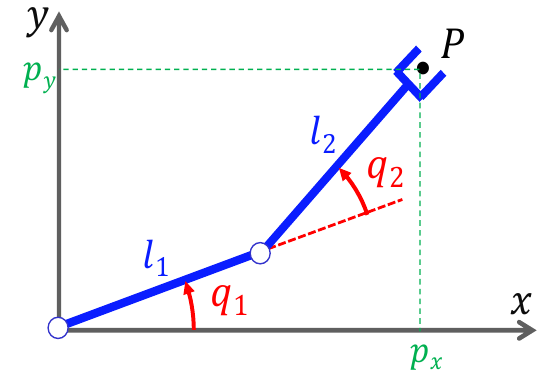
\includegraphics[width=\linewidth,height=0.67\textheight,keepaspectratio]{dl11_p033_arm.png}
        \end{column}
        \begin{column}{0.38\textwidth}
            \vspace{2mm}
            \normalsize
            Two links: $l_1,l_2$.\\[2mm]
            Joint angles: $q_1,q_2$.\\[2mm]
            $P$ is the selected end-effector point.\\[2mm]
            \scriptsize\textbf{Notation.} $l_i$: link length; $q_i$: joint angle; $P$: task point.\\[3mm]
            \alert{If $P$ is reachable, can it move in every direction?}
        \end{column}
    \end{columns}
\end{frame}

\begin{frame}[t]{Position workspace of point $P$}
    \begin{columns}[T,onlytextwidth]
        \begin{column}{0.53\textwidth}
            \normalsize
            \[
                r^2=l_1^2+l_2^2+2l_1l_2\cos q_2
            \]
            Since $-1\leq\cos q_2\leq1$,
            \[
                |l_1-l_2|\leq r\leq l_1+l_2.
            \]
            If $l_1=l_2$, the inner radius is zero.\\[2mm]
            \small\textbf{Notation.} $r$: distance from the base to $P$.
        \end{column}
        \begin{column}{0.44\textwidth}
            \centering
            \begin{tikzpicture}[scale=1.25]
                \fill[blue!13,even odd rule] (0,0) circle (2.1) (0,0) circle (0.65);
                \draw[blue,thick] (0,0) circle (2.1);
                \draw[blue,thick] (0,0) circle (0.65);
                \fill (0,0) circle (2pt);
                \node[right] at (0.6,0.55) {$|l_1-l_2|$};
                \node[right] at (1.45,1.45) {$l_1+l_2$};
            \end{tikzpicture}
        \end{column}
    \end{columns}
    \scriptsize\alert{Question: On the outer boundary, can $P$ move radially outward instantaneously?}
\end{frame}

\begin{frame}[c]
    \centering
    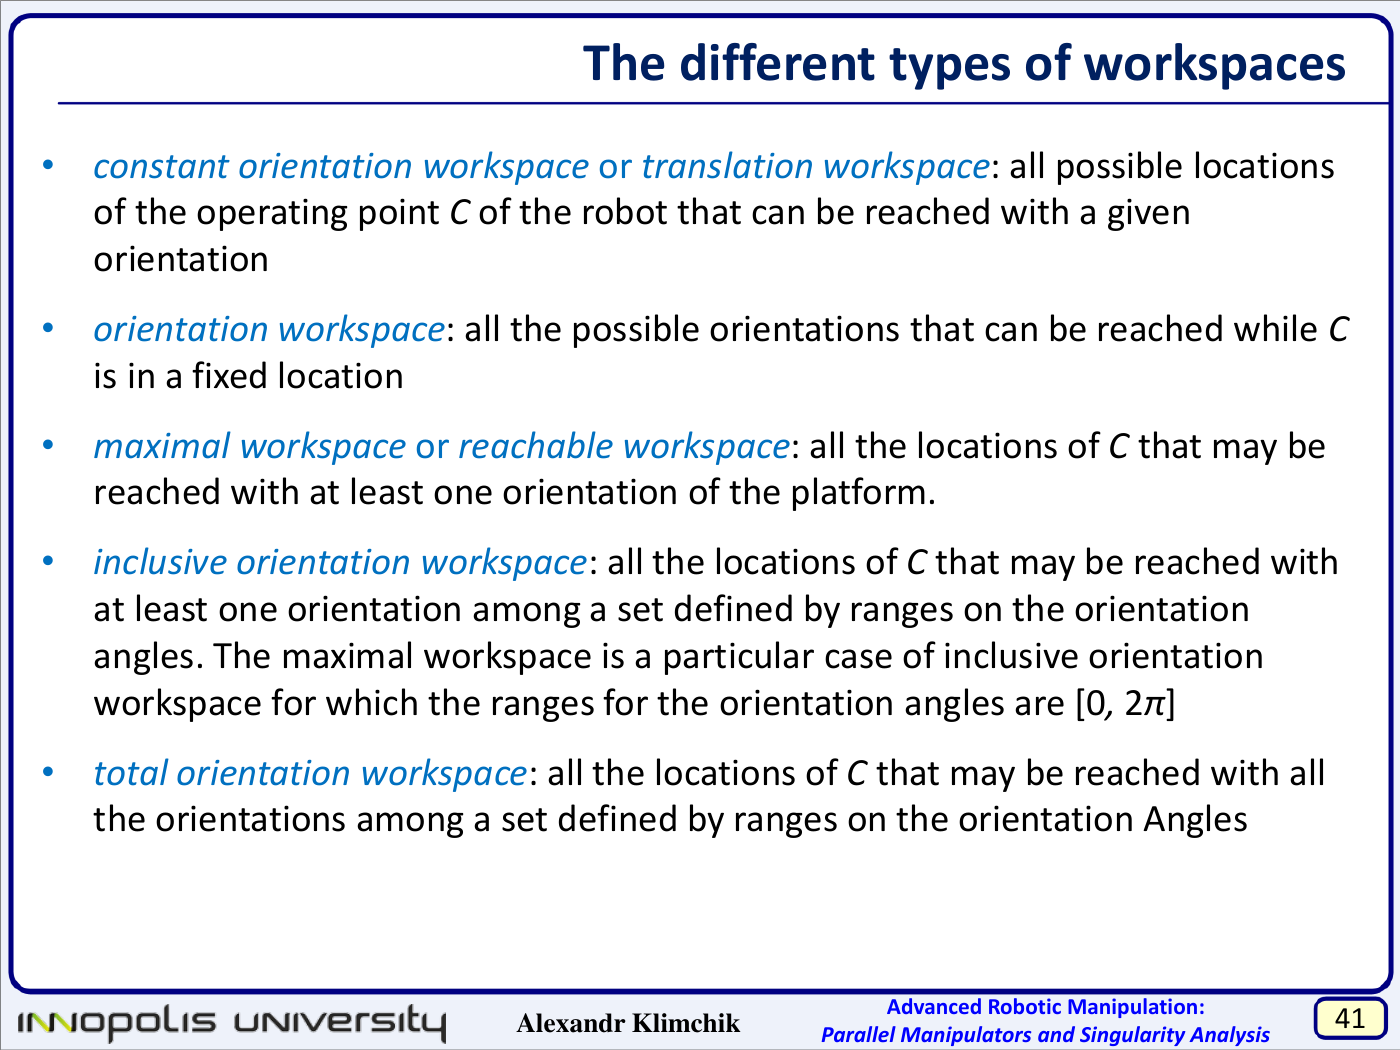
\includegraphics[width=\textwidth,height=0.8\paperheight,keepaspectratio]{kl_l4_p041_full.png}
\end{frame}

\begin{frame}[c]
    \centering
    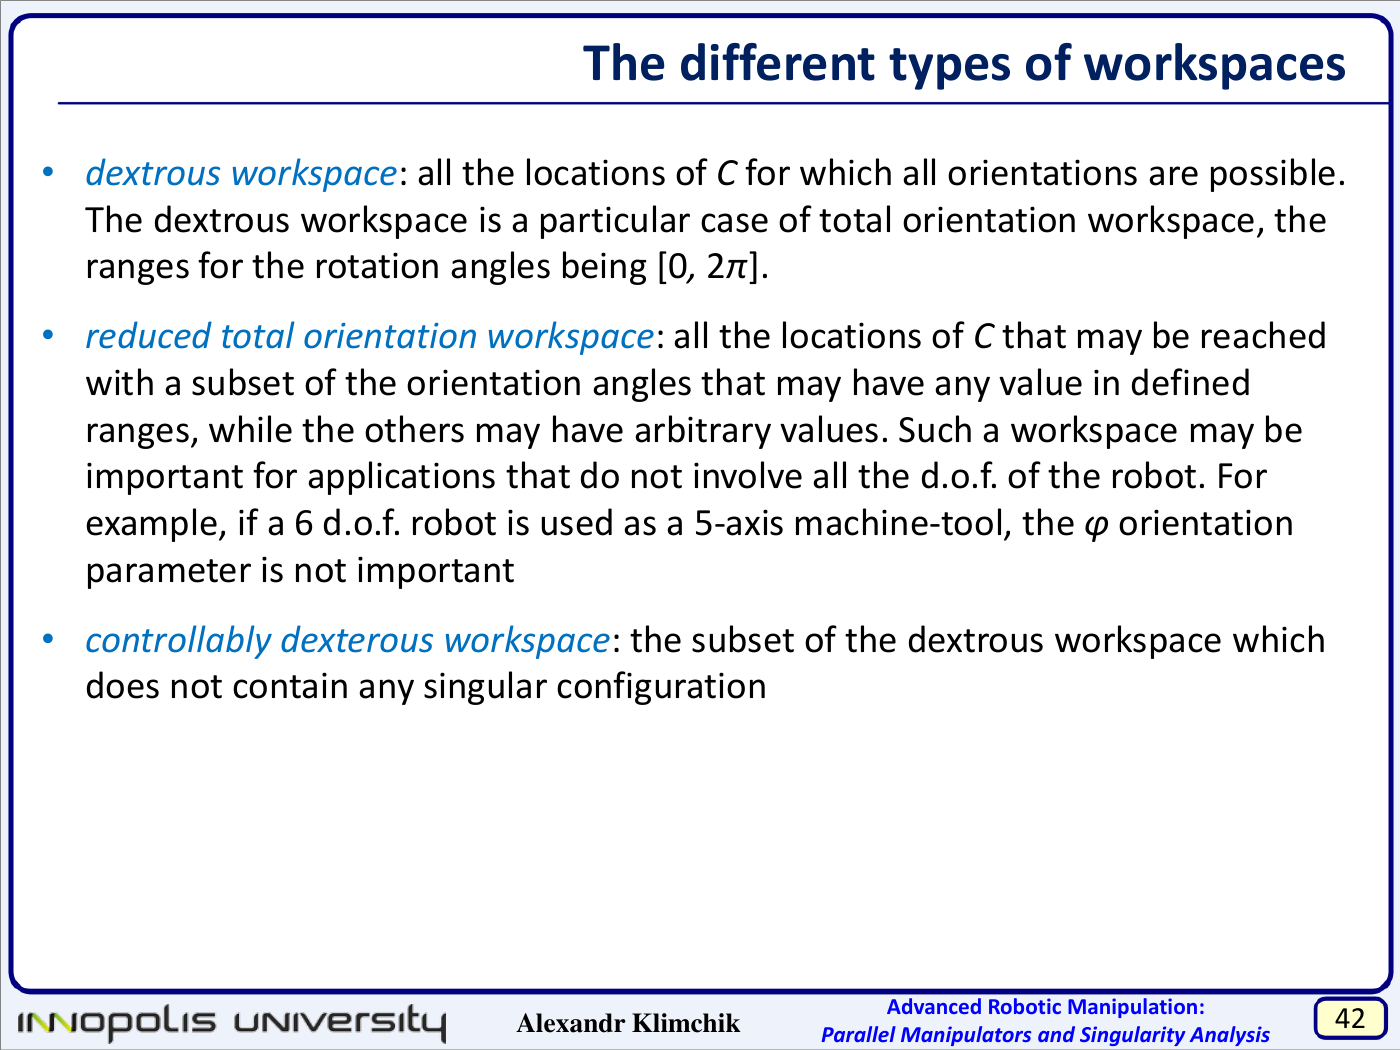
\includegraphics[width=\textwidth,height=0.8\paperheight,keepaspectratio]{kl_l4_p042_full.png}
\end{frame}

\begin{frame}[t]{Why are these workspaces different?}
    \framesubtitle{Planar 3R arm: two 1 m links and a tool of length $d=0.4$ m}
    \begin{columns}[T,onlytextwidth]
        \begin{column}{0.48\textwidth}
            \centering
            \begin{tikzpicture}[scale=1.45,>=Latex]
                \coordinate (O) at (0,0);
                \coordinate (W) at (2.0,0.65);
                \coordinate (P) at (2.75,1.02);
                \draw[->,gray] (-0.2,0)--(3.1,0) node[right] {$x$};
                \draw[->,gray] (0,-0.2)--(0,1.9) node[above] {$y$};
                \draw[blue,very thick] (O)--(0.9,0.85)--(W);
                \draw[orange,very thick] (W)--(P);
                \fill (O) circle (2pt) node[below left] {$O$};
                \fill (W) circle (2pt) node[below] {$W$};
                \fill[orange] (P) circle (2.5pt) node[above] {$P$};
                \node[orange,above] at (2.40,0.83) {$d\,u(\varphi)$};
            \end{tikzpicture}
            \[
                W=P-d\,u(\varphi),\qquad \|W\|\leq2.
            \]
        \end{column}
        \begin{column}{0.49\textwidth}
            \scriptsize
            \begin{block}{Fixed orientation}
                $\|P-d\,u(\varphi)\|\leq2$: a shifted radius-2 m circle.
            \end{block}
            \begin{block}{At least one $\varphi$ exists}
                $\min_\varphi\|P-d\,u(\varphi)\|=|\|P\|-d|$; maximum: $\|P\|\leq2.4$ m.
            \end{block}
            \begin{block}{Every $\varphi$ works}
                $\max_\varphi\|P-d\,u(\varphi)\|=\|P\|+d$; dextrous: $\|P\|\leq1.6$ m.
            \end{block}
            \textbf{Notation.} $O$: base; $W$: wrist; $d$: tool length; $u(\varphi)$: unit direction.
        \end{column}
    \end{columns}
\end{frame}

\begin{frame}[t]{Computing a Workspace: FK and IK}
    \framesubtitle{The first choice is which direction to solve the kinematic map}
    \small
    \begin{columns}[T,onlytextwidth]
        \begin{column}{0.49\textwidth}
            \begin{block}{Sample joint configurations (FK)}
                Compute $p=f(q)$ for many joint samples and mark the resulting poses.
            \end{block}
            \begin{itemize}
                \item Simple; no inverse kinematics is needed.
                \item Samples cover task space unevenly and may miss a boundary.
            \end{itemize}
        \end{column}
        \begin{column}{0.49\textwidth}
            \begin{block}{Test task-space poses (IK)}
                Select poses $p$ and ask whether an allowed $q$ solves $f(q)=p$.
            \end{block}
            \begin{itemize}
                \item Tests chosen poses and can count solution branches.
                \item Needs complete, reliable IK; numerical failure alone does not prove a pose unreachable.
            \end{itemize}
        \end{column}
    \end{columns}
\end{frame}

\begin{frame}[t]{Describing a Workspace: Geometry and Grid}
    \framesubtitle{The second choice is how to describe or test the reachable set}
    \begin{columns}[T,onlytextwidth]
        \begin{column}{0.49\textwidth}
            \begin{block}{Geometric computation}
                $\|P-d\,u(\varphi)\|\leq2$ gives an exact circle boundary for this simple arm; complex limits make analytic geometry harder.
            \end{block}
            \centering
            \begin{tikzpicture}[scale=0.48]
                \draw[blue,very thick] (0,0) circle (2);
                \fill[orange] (1.8,0.5) circle (3pt);
            \end{tikzpicture}
        \end{column}
        \begin{column}{0.49\textwidth}
            \begin{block}{Grid computation}
                Test regular nodes, using a geometric condition or IK. Limits and branch counts fit naturally, but the boundary is approximate.
            \end{block}
            \centering
            \begin{tikzpicture}[scale=0.48]
                \foreach \x in {-1.8,-1.4,-1.0,-0.6,-0.2,0.2,0.6,1.0,1.4,1.8} {
                    \foreach \y in {-1.8,-1.4,-1.0,-0.6,-0.2,0.2,0.6,1.0,1.4,1.8} {
                        \pgfmathtruncatemacro{\inside}{(\x*\x+\y*\y)<4}
                        \ifnum\inside=1
                            \fill[blue!25] (\x-0.2,\y-0.2) rectangle (\x+0.2,\y+0.2);
                        \fi
                    }
                }
                \draw[step=0.4,gray!40,very thin] (-2.1,-2.1) grid (2.1,2.1);
                \draw[blue,dashed] (0,0) circle (2);
                \fill[orange] (1.8,0.5) circle (3pt);
            \end{tikzpicture}
        \end{column}
    \end{columns}
    \scriptsize Geometry checks the answer; a grid makes broader cases computable. In $D$ dimensions, node count is of order $(L/h)^D$. \textbf{Notation.} $L$: span; $h$: spacing; $D$: dimension.
\end{frame}

\begin{frame}[t]{Explore workspaces in the model}
    \framesubtitle{One geometry, different orientation requirements for point $P$}
    \begin{enumerate}
        \item Set $P=(2.2,0)$ m. Is it reachable for every tool orientation?
        \item Compare \textbf{at least one} with \textbf{every} orientation in $[-60^\circ,60^\circ]$.
        \item Switch one workspace between geometric and grid computation. What changes?
    \end{enumerate}
    \vspace{6mm}
    \begin{block}{Open the interactive model}
        \href{http://localhost:8765/workspace.html}{\texttt{http://localhost:8765/workspace.html}}
    \end{block}
    \vspace{3mm}
    \large The maximum workspace $\supseteq$ the dextrous workspace. A reachable position still does not guarantee the required instantaneous velocity.
\end{frame}

\begin{frame}[c]
    \centering
    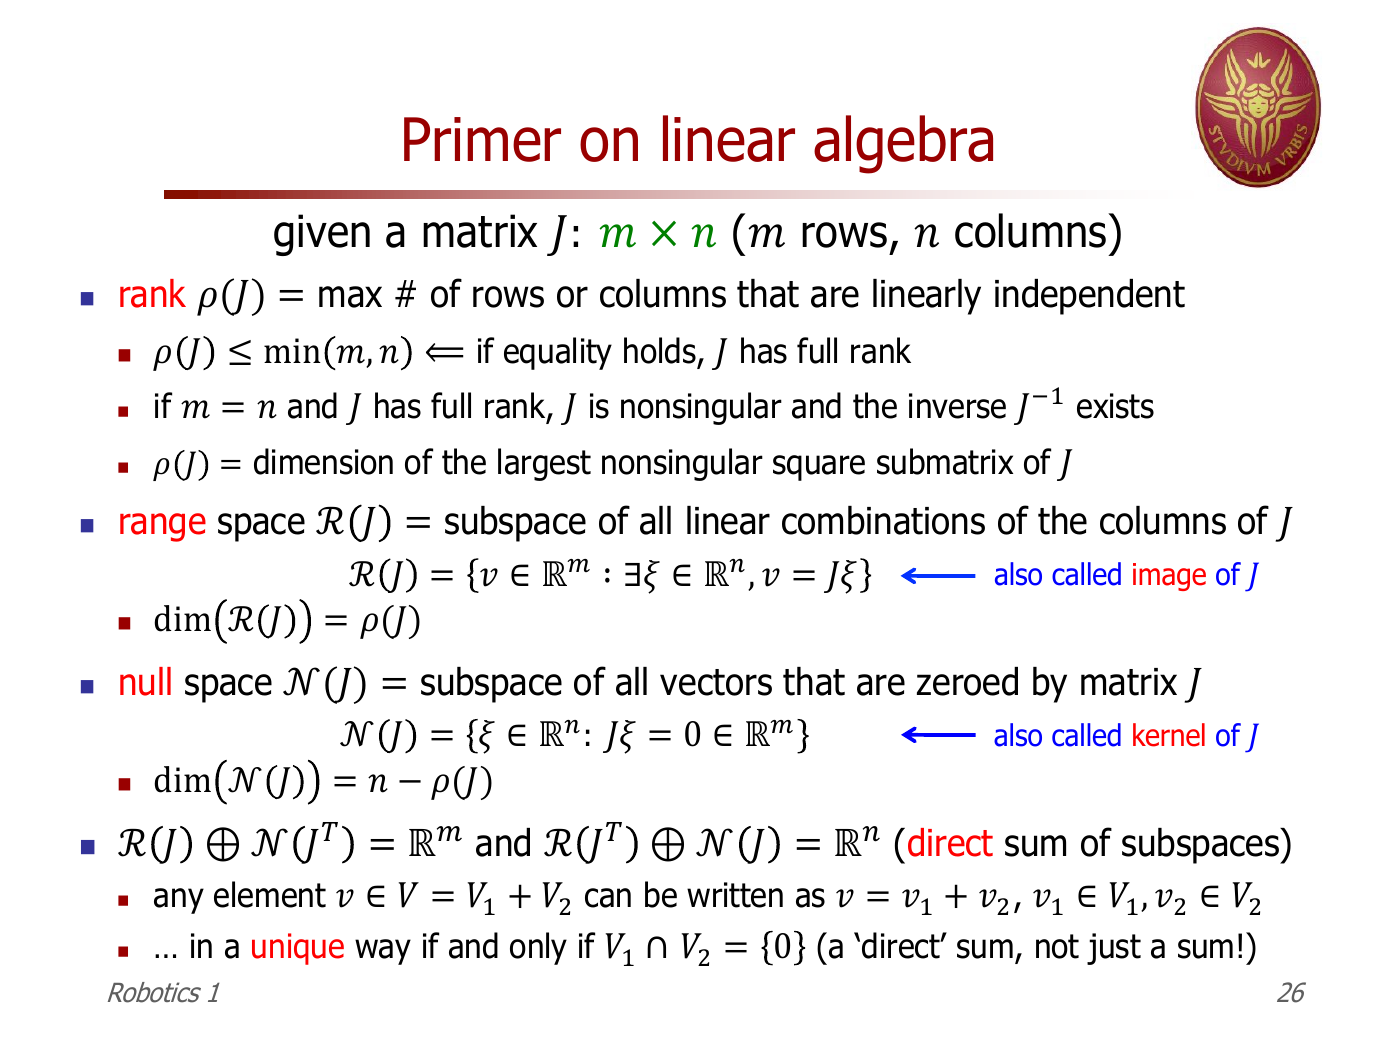
\includegraphics[width=\textwidth,height=0.8\paperheight,keepaspectratio]{dl11_p026_full.png}
\end{frame}

\begin{frame}[c]
    \centering
    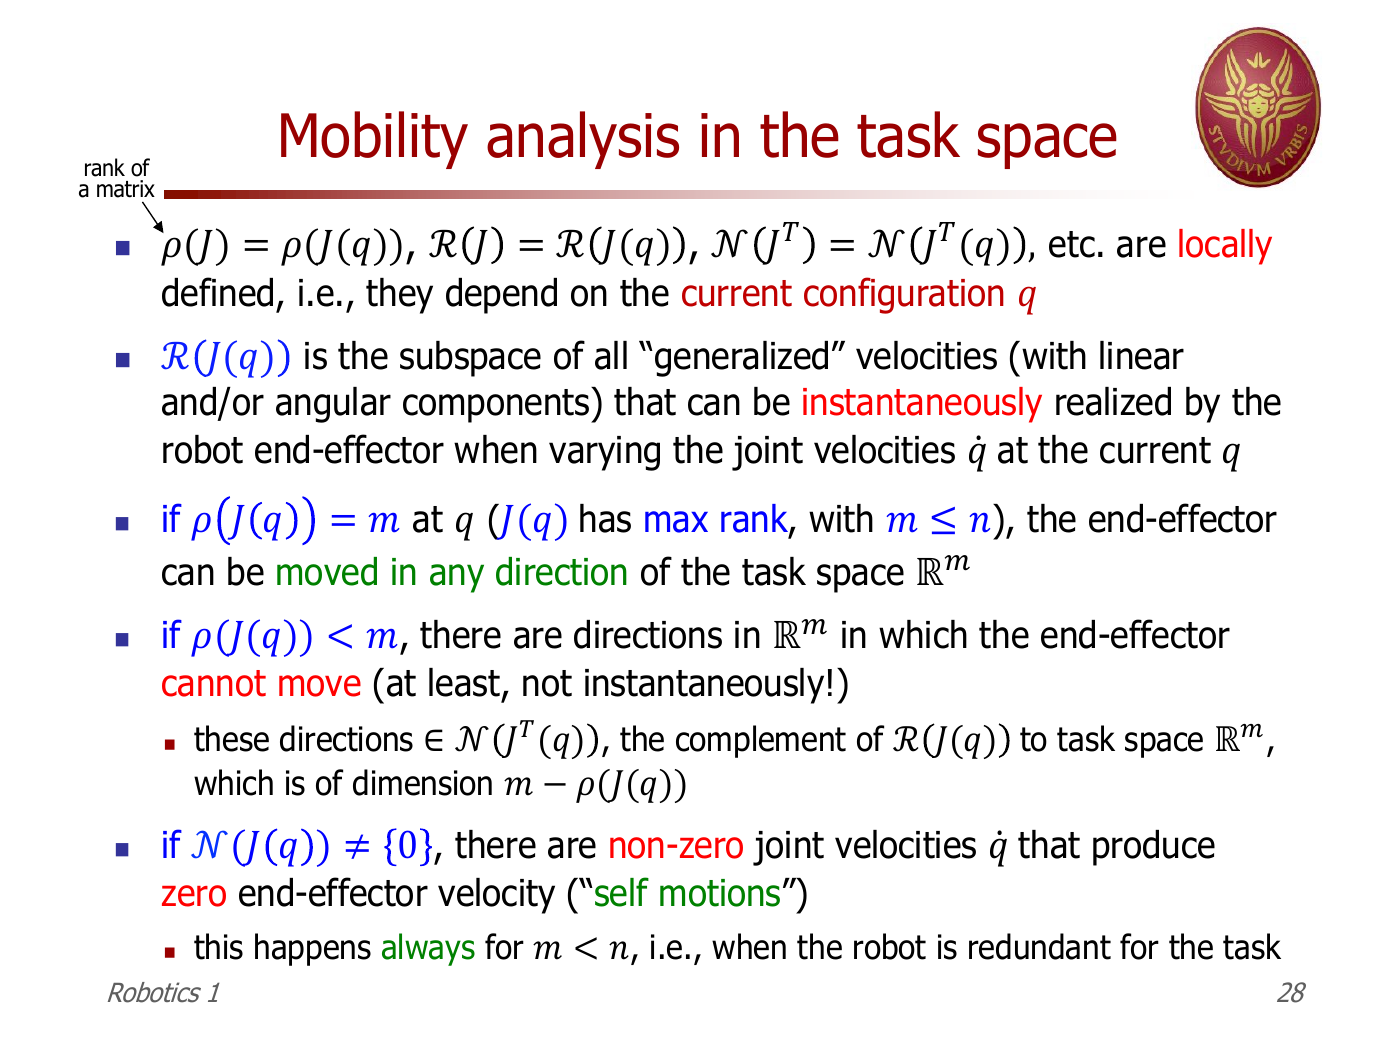
\includegraphics[width=\textwidth,height=0.8\paperheight,keepaspectratio]{dl11_p028_full.png}
\end{frame}

\begin{frame}[c]
    \centering
    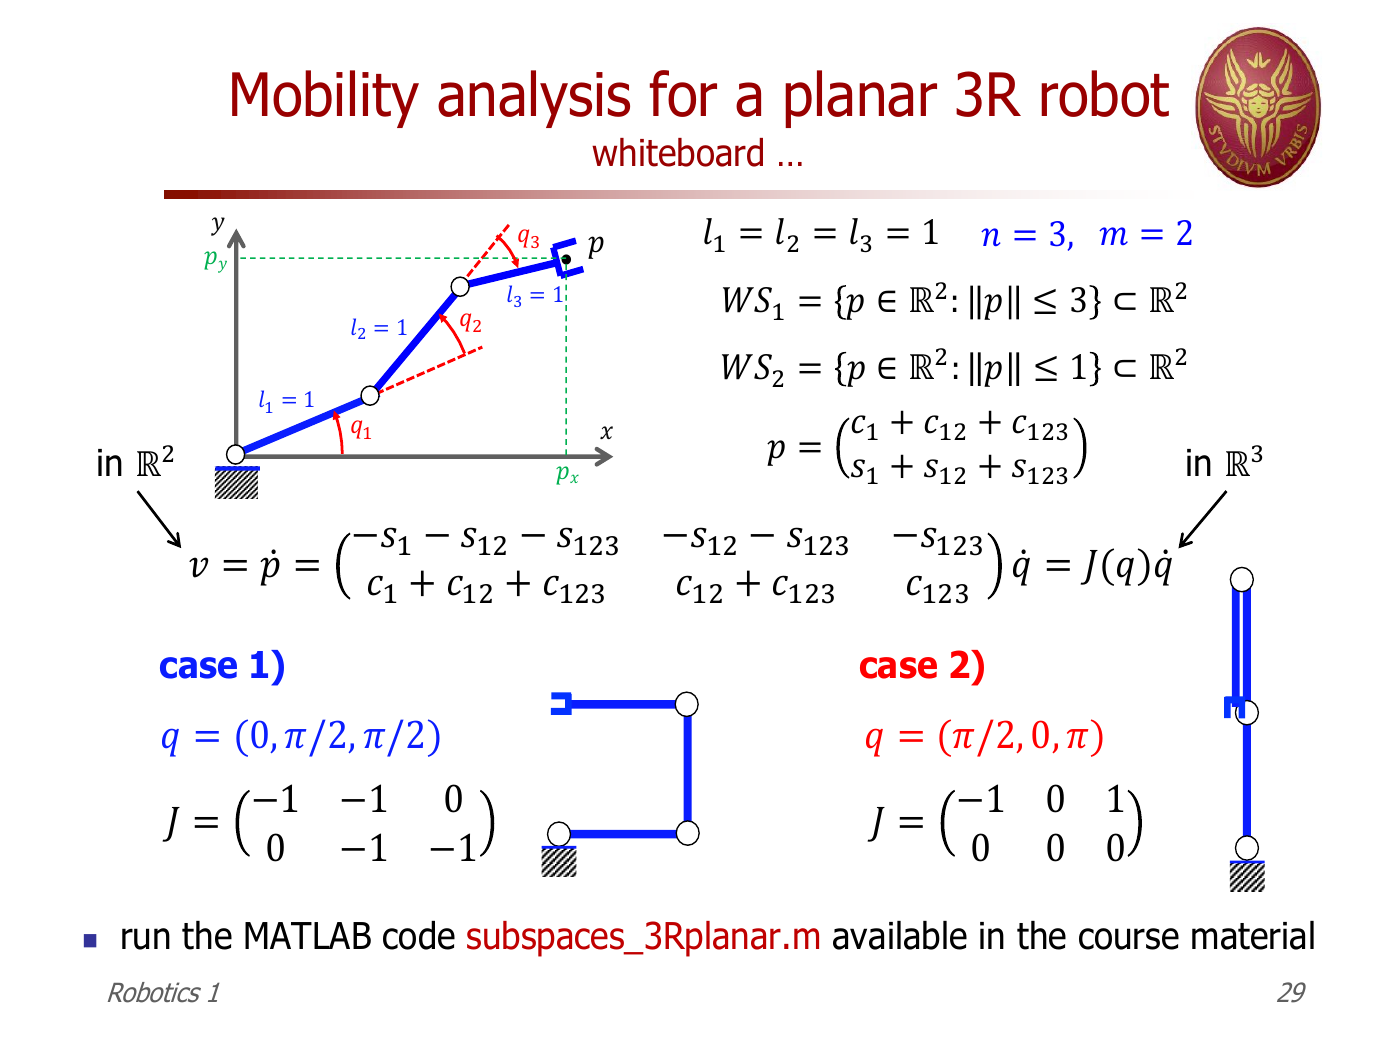
\includegraphics[width=\textwidth,height=0.8\paperheight,keepaspectratio]{dl11_p029_full.png}
\end{frame}

\begin{frame}[c]
    \centering
    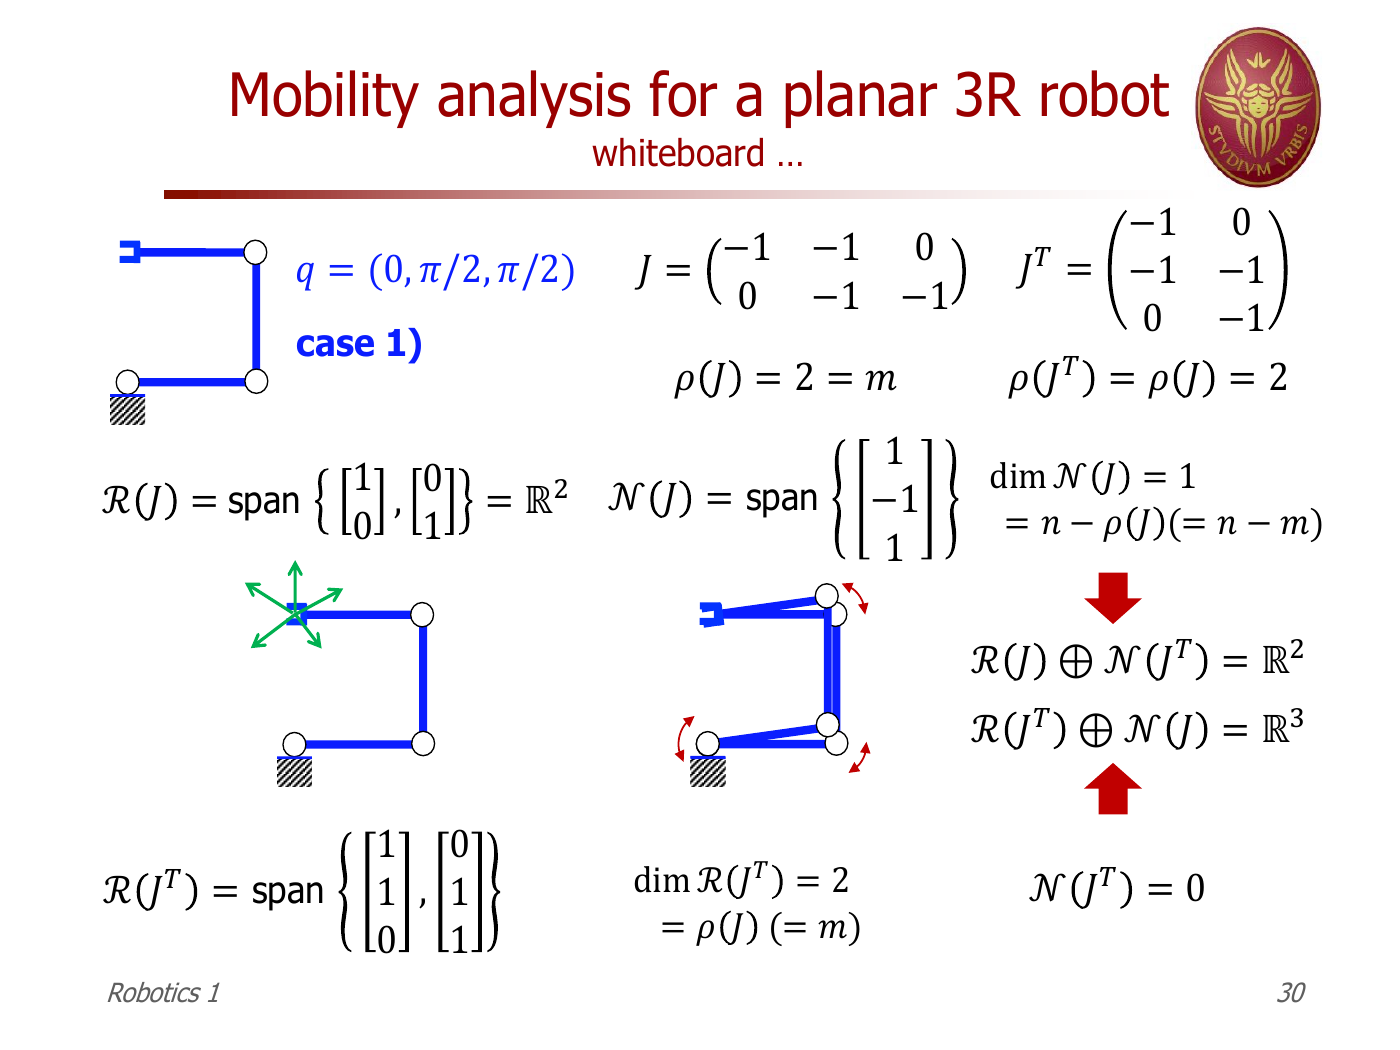
\includegraphics[width=\textwidth,height=0.8\paperheight,keepaspectratio]{dl11_p030_full.png}
\end{frame}

\begin{frame}[c]
    \centering
    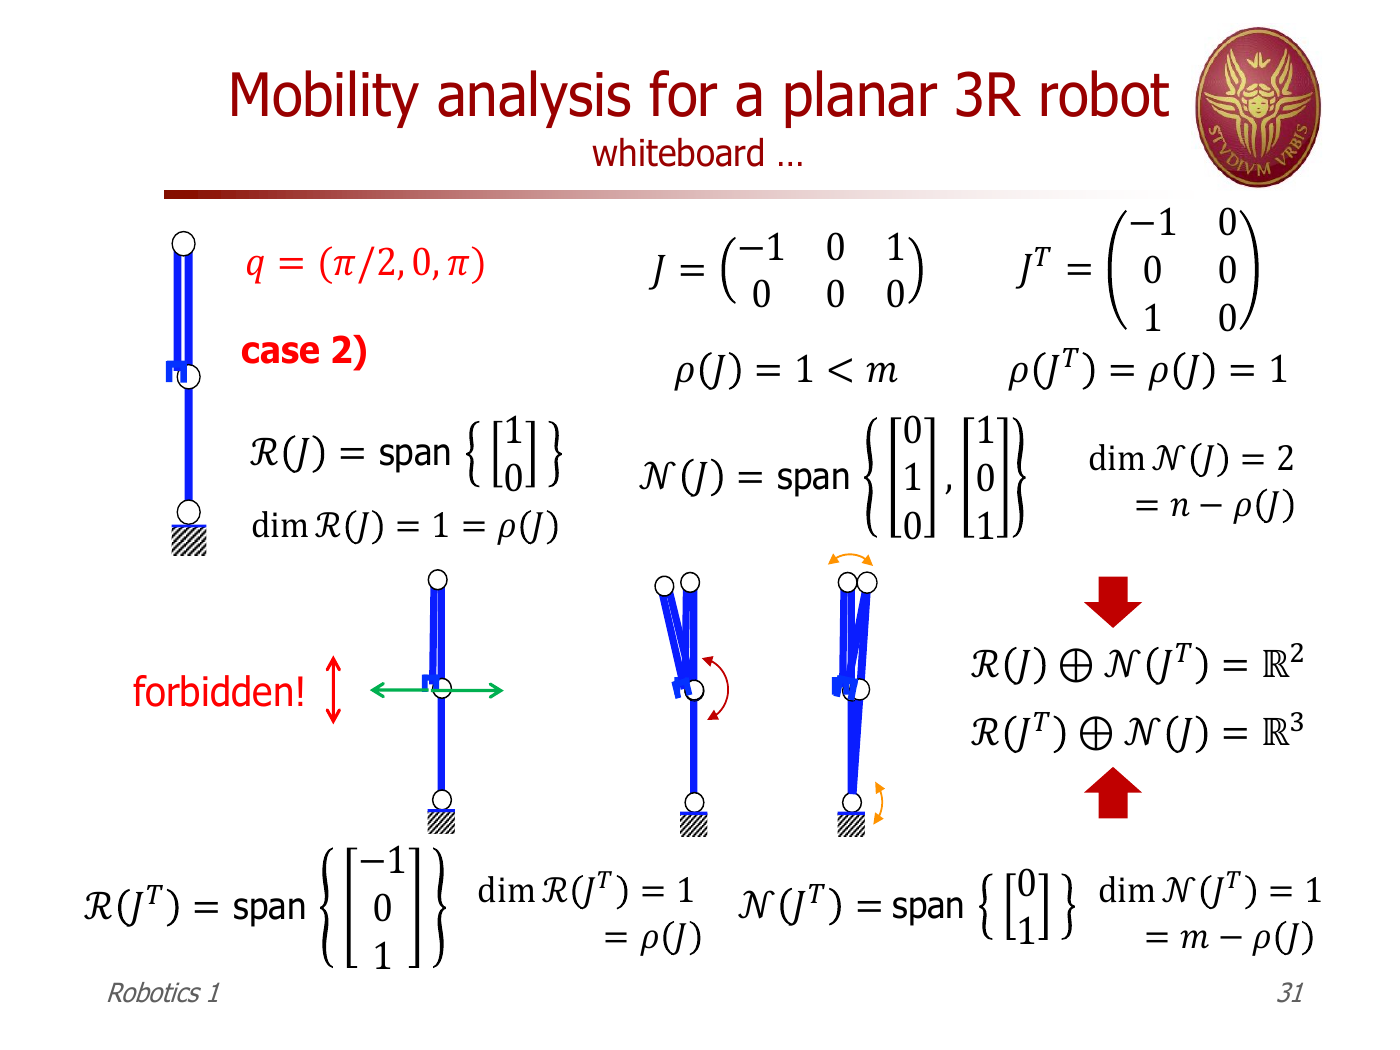
\includegraphics[width=\textwidth,height=0.8\paperheight,keepaspectratio]{dl11_p031_full.png}
\end{frame}

\begin{frame}[c]
    \centering
    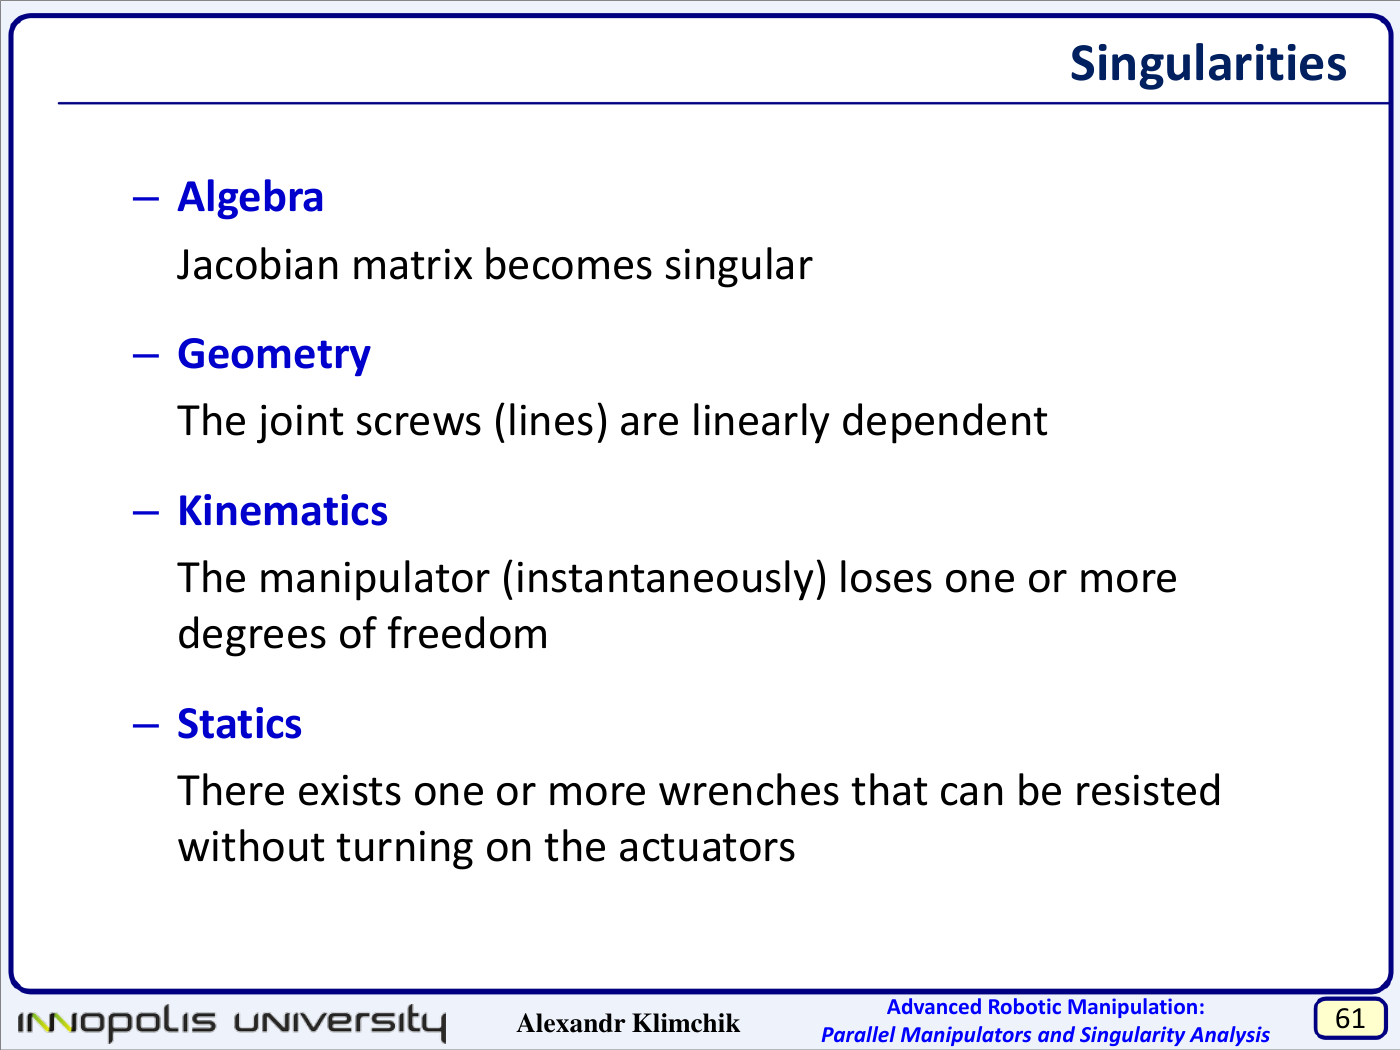
\includegraphics[width=\textwidth,height=0.8\paperheight,keepaspectratio]{kl_l4_p061_full.png}
\end{frame}

\begin{frame}[c]
    \centering
    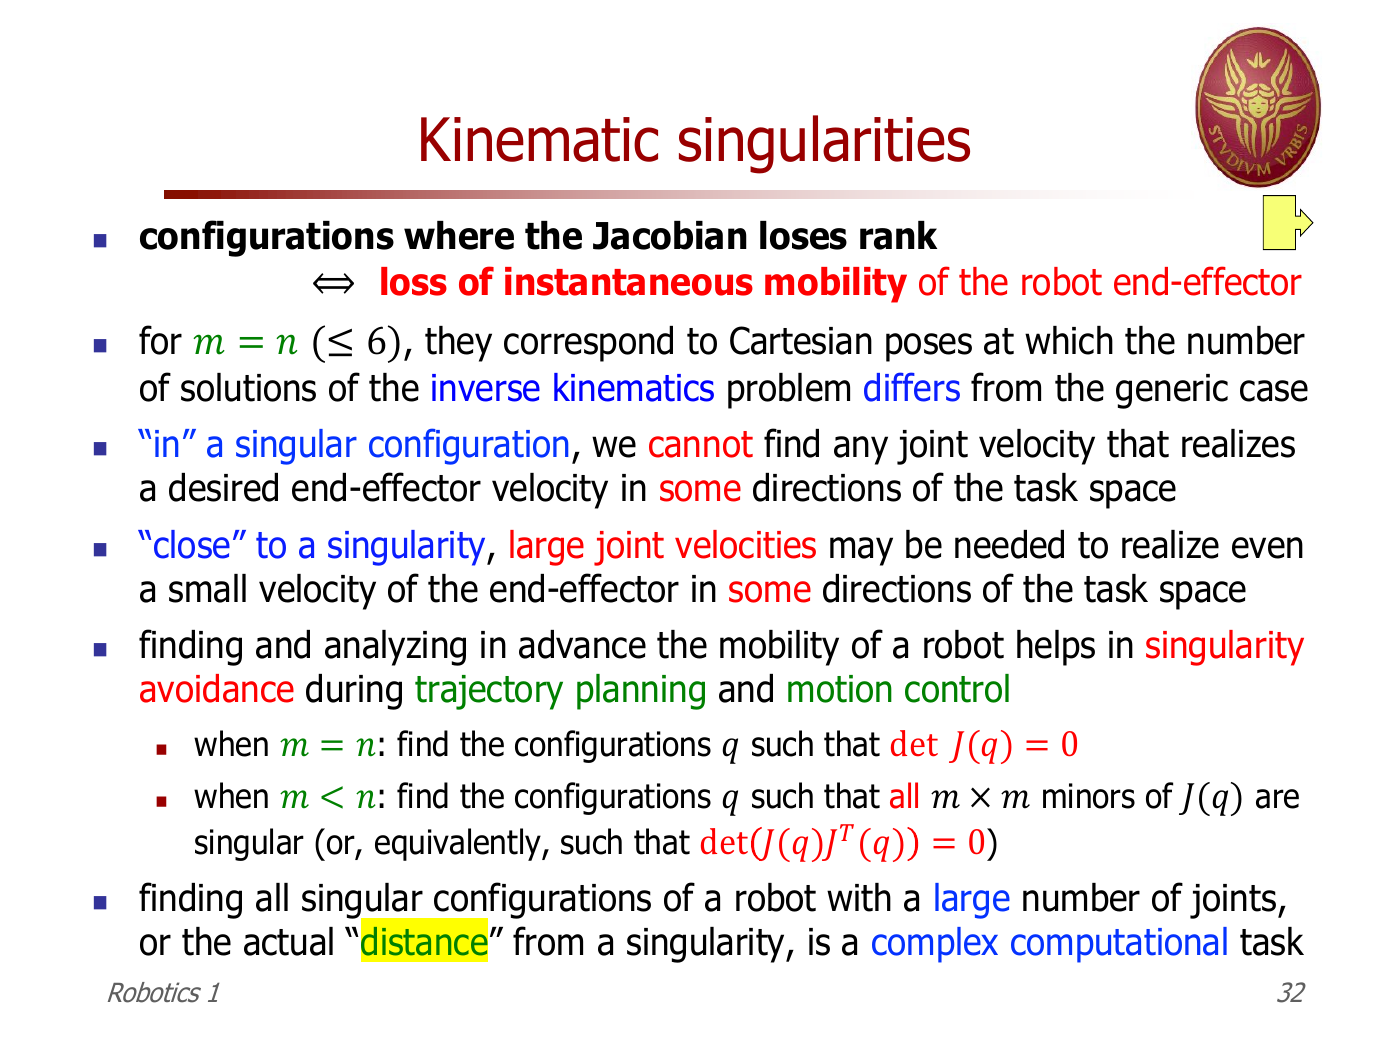
\includegraphics[width=\textwidth,height=0.8\paperheight,keepaspectratio]{dl11_p032_full.png}
\end{frame}

\begin{frame}[t]{Derive the 2R Jacobian}
    \framesubtitle{Linear velocity of point $P$: $\dot p=J(q)\dot q$}
    \normalsize
    \[
        x_P=l_1\cos q_1+l_2\cos(q_1+q_2)
    \]
    \[
        y_P=l_1\sin q_1+l_2\sin(q_1+q_2)
    \]
    \[
        J(q)=\frac{\partial(x_P,y_P)}{\partial(q_1,q_2)}
        =\begin{bmatrix}?&?\\[3mm]
        ?&?\end{bmatrix}
    \]
    \scriptsize\textbf{Notation.} $p=(x_P,y_P)^{\mathsf T}$: position of $P$; $q=(q_1,q_2)^{\mathsf T}$: joint coordinates; a dot denotes velocity; $J(q)$ maps joint velocity to point velocity.
    \scriptsize\alert{\textbf{Question.} Each column: velocity of $P$ from unit speed of its joint?}
\end{frame}

\begin{frame}[t]{What is lost in the stretched pose?}
    \framesubtitle{$l_1=l_2=1$ m, $q_1=q_2=0$}
    \begin{columns}[T,onlytextwidth]
        \begin{column}{0.47\textwidth}
            \normalsize
            \[
                J=\begin{bmatrix}0&0\\2&1\end{bmatrix},
                \quad
                \begin{bmatrix}\dot x_P\\\dot y_P\end{bmatrix}
                =\begin{bmatrix}0\\2\dot q_1+\dot q_2\end{bmatrix}.
            \]
            $\operatorname{rank}J=1$.\\
            The image of $J$ is the vertical line.
        \end{column}
        \begin{column}{0.49\textwidth}
            \normalsize
            \begin{block}{Command to the right}
                $\dot p=(0.5,0)$ m/s.\par
                \alert{There is no solution for $\dot q$.}
            \end{block}
            \begin{block}{Command upward}
                $\dot p=(0,0.5)$ m/s.\par
                $2\dot q_1+\dot q_2=0.5$.\\
                Many solutions.
            \end{block}
        \end{column}
    \end{columns}
    \small A workspace-boundary point may still lack the required \emph{instantaneous} velocity.
\end{frame}

\begin{frame}[t]{Test the 2R singularity in the model}
    \framesubtitle{Point position on the left, attainable linear velocities on the right}
    \begin{enumerate}
        \item Keep the orange arrow pointing right. Change $q_2$: $60^\circ\to5^\circ\to0^\circ$.
        \item What happens to the blue velocity region and required $\|\dot q\|$?
        \item At $q_2=0$, turn the arrow upward. Why does the result change?
        \item Compare the metrics shown by the model.
    \end{enumerate}
    \vspace{3mm}
    \begin{block}{Open the interactive model}
        \href{http://localhost:8765/}{\texttt{http://localhost:8765/}}
    \end{block}
    The blue region is $\{J\dot q:\|\dot q\|\leq1\}$; the orange-arrow tip is the requested velocity $\|\dot p\|=0.5$ m/s.
\end{frame}

\begin{frame}[c]
    \centering
    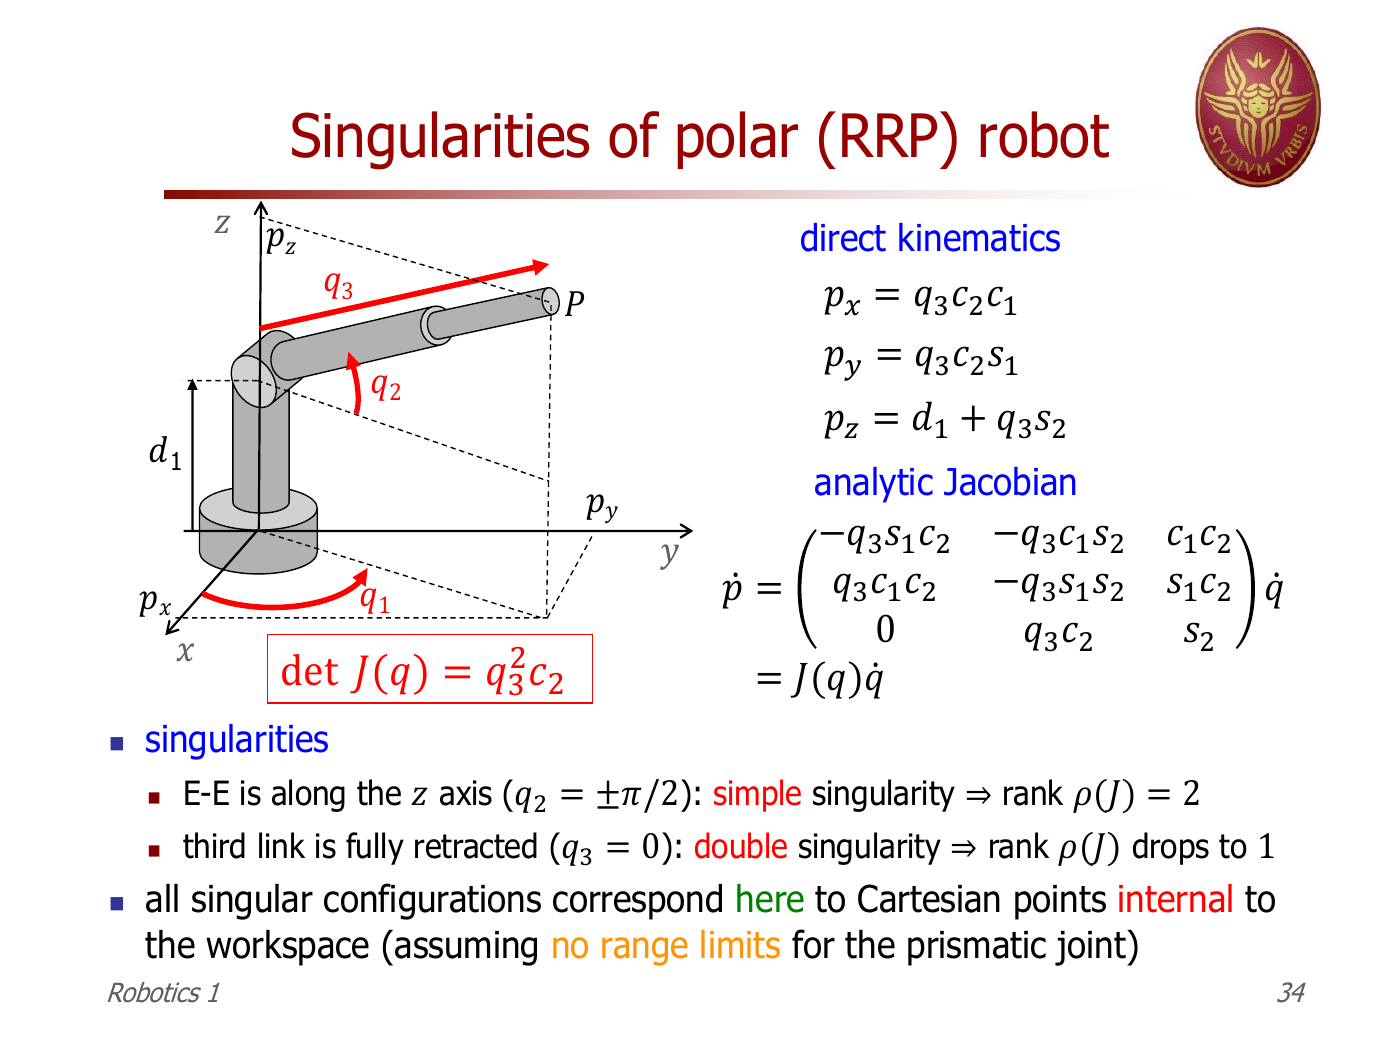
\includegraphics[width=\textwidth,height=0.8\paperheight,keepaspectratio]{dl11_p034_full.png}
\end{frame}

\begin{frame}[c]
    \centering
    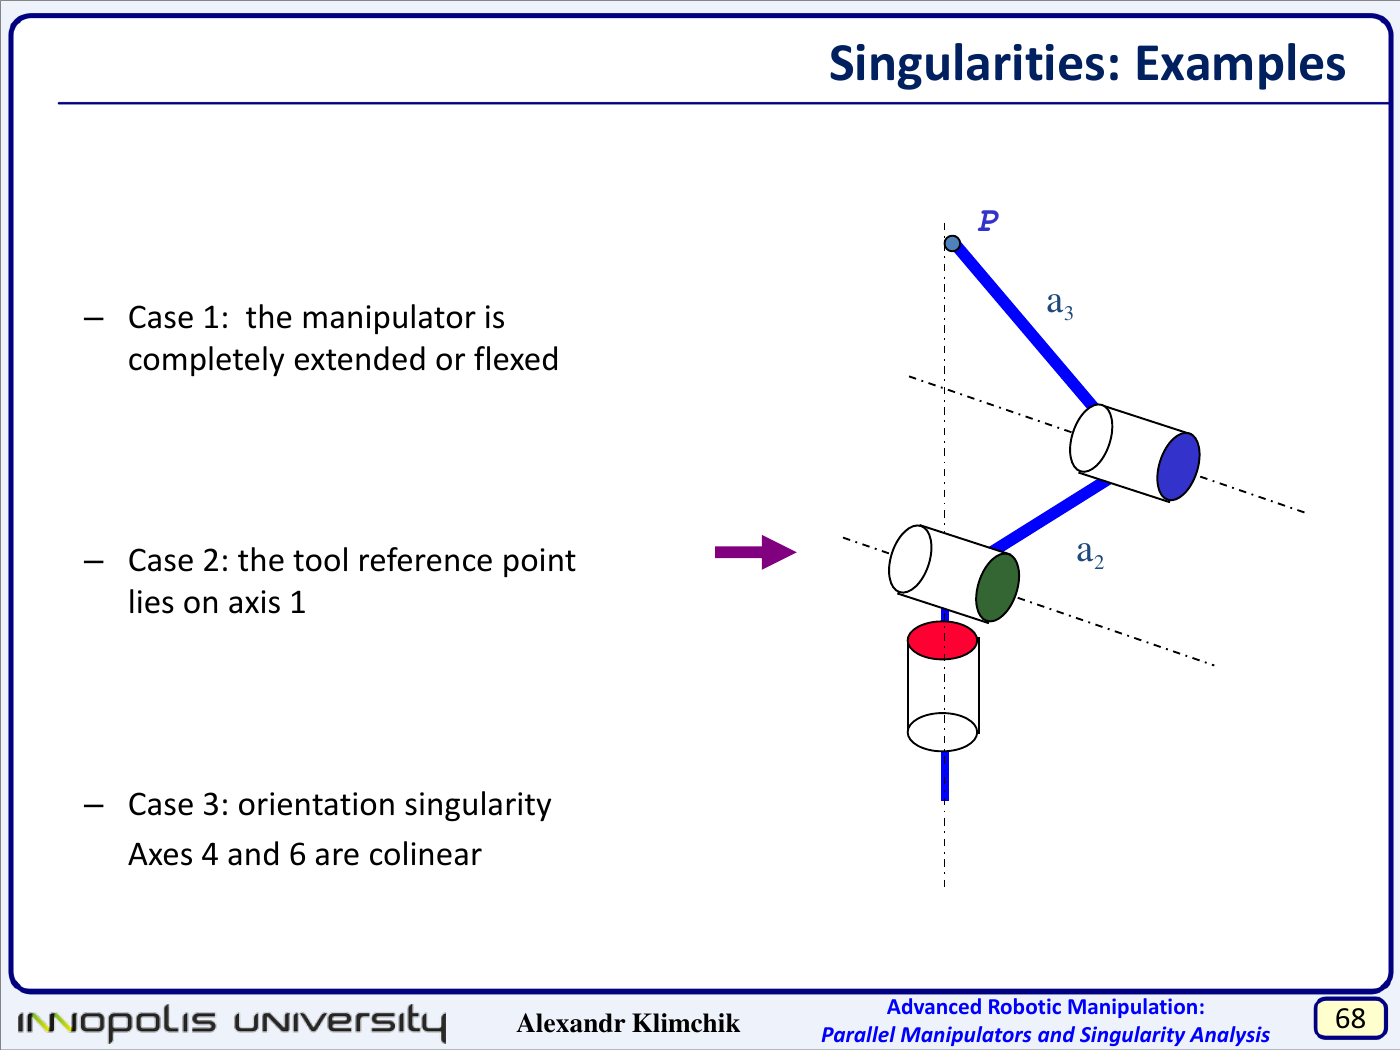
\includegraphics[width=\textwidth,height=0.8\paperheight,keepaspectratio]{kl_l4_p068_full.png}
\end{frame}

\begin{frame}[c]
    \centering
    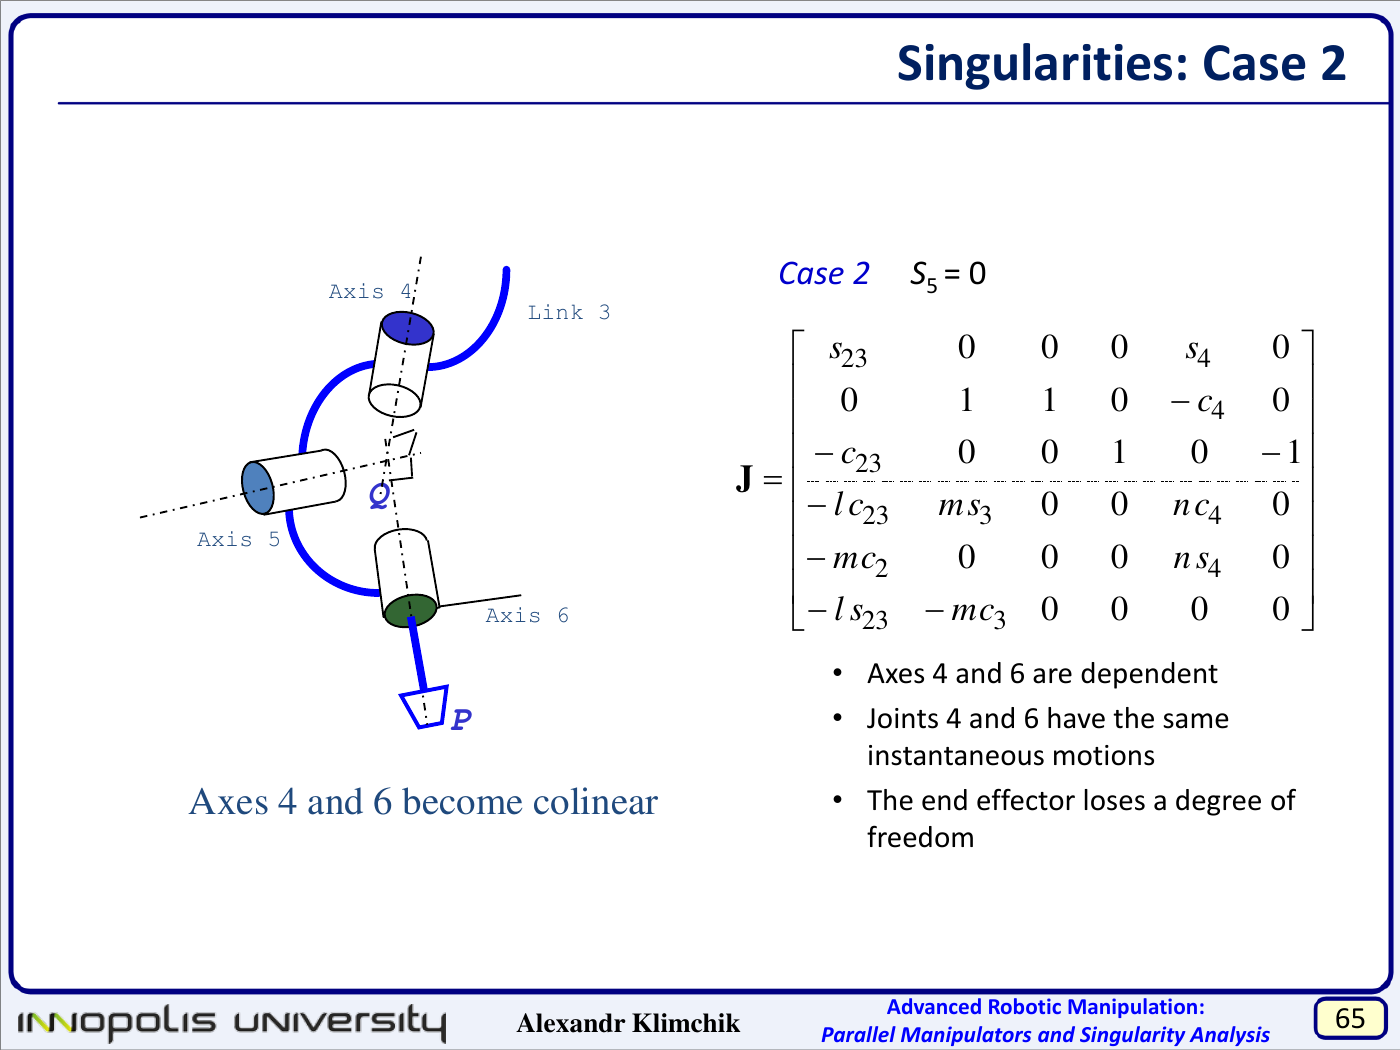
\includegraphics[width=\textwidth,height=0.8\paperheight,keepaspectratio]{kl_l4_p065_full.png}
\end{frame}

\begin{frame}[c]
    \centering
    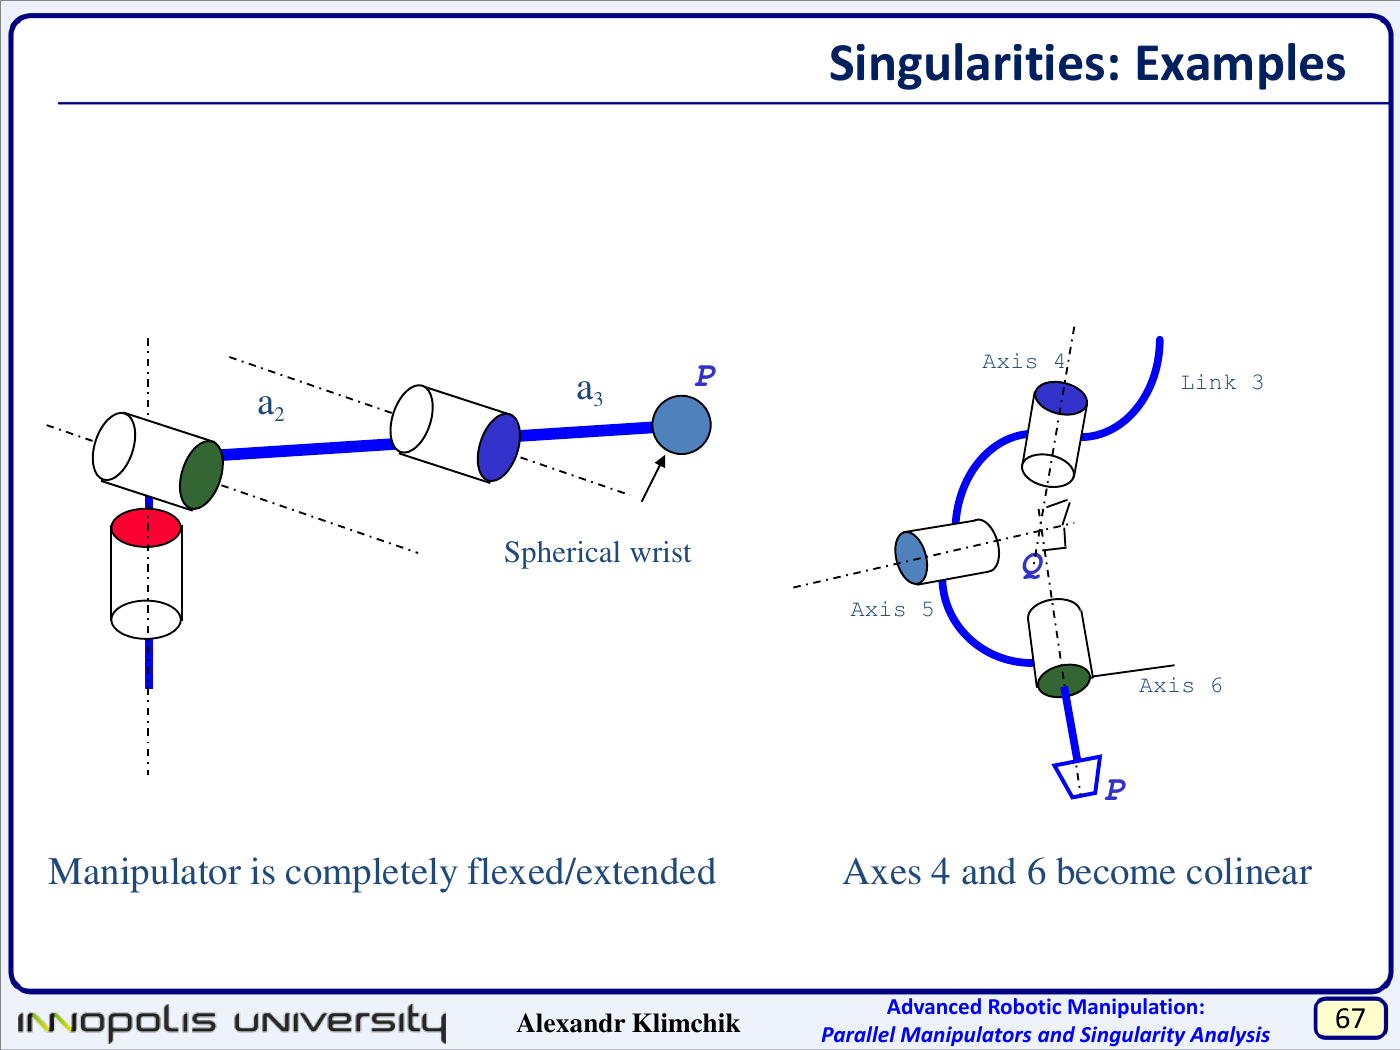
\includegraphics[width=\textwidth,height=0.8\paperheight,keepaspectratio]{kl_l4_p067_full.png}
\end{frame}

\begin{frame}[t]{How close is a singularity?}
    \framesubtitle{Different metrics answer different questions}
    \small
    \begin{tabularx}{\textwidth}{>{\raggedright\arraybackslash}p{0.26\textwidth} >{\raggedright\arraybackslash}p{0.34\textwidth} X}
        \toprule
        Metric & 2R formula & Meaning \\
        \midrule
        Pose distance & $\min(|q_2|,\,|\pi-|q_2||)$ & Angular distance in configuration space \\
        Manipulability & $w=\sqrt{\det(JJ^{\mathsf T})}=\prod_i\sigma_i$ & Velocity-ellipse area is proportional to $w$ \\
        Weak direction & $\sigma_{\min}(J)$ & Smallest velocity stretch \\
        Anisotropy & $1/\kappa_2(J)=\sigma_{\min}/\sigma_{\max}$ & Minor-to-major ellipse-axis ratio \\
        \bottomrule
    \end{tabularx}
    \scriptsize\textbf{Notation.} $\sigma_i$: singular values of $J$; $\sigma_{\min}$ and $\sigma_{\max}$: smallest and largest; $w$: manipulability; $\kappa_2$: 2-norm condition number.
    \begin{block}{Caution}
        Comparing linear and angular components of a full Jacobian requires an explicit length scale.
    \end{block}
\end{frame}

\begin{frame}[t]{Why one determinant is not enough}
    \framesubtitle{Mathematical matrices, not models of specific robots}
    \normalsize
    \small\textbf{Notation.} $J_A$ and $J_B$ are comparison matrices.
    \[
        J_A=\begin{bmatrix}10&0\\0&0.1\end{bmatrix},
        \qquad
        J_B=\begin{bmatrix}1&0\\0&1\end{bmatrix}
    \]
    \small
    \begin{center}
        \footnotesize
        \begin{tabular}{lcc}
            \toprule
            & $J_A$ & $J_B$ \\
            \midrule
            $w=|\det J|$ & $1$ & $1$ \\
            $\sigma_{\min}$ & $0.1$ & $1$ \\
            $1/\kappa_2$ & $0.01$ & $1$ \\
            Required $\|\dot q\|$ for $\dot p=(0,1)^{\mathsf T}$ & $10$ & $1$ \\
            \bottomrule
        \end{tabular}
    \end{center}
    \vspace{-4mm}
    \footnotesize Both matrices are nonsingular; their equal-area ellipses hide different weak directions. For $\dot p=(0,1)^{\mathsf T}$, $\dot q_A=(0,10)^{\mathsf T}$ and $\dot q_B=(0,1)^{\mathsf T}$. Compare $\sigma_{\min}$ and conditioning with consistent units and scales.
\end{frame}

\begin{frame}[t]{What should an engineer do?}
    \small
    \begin{block}{Scenario}
        A robot drives a tool point along a line near a stretched pose. A small linear velocity in the weak direction can demand an infeasible joint speed.
    \end{block}
    \begin{itemize}
        \item Change the configuration, approach, tool orientation, or part placement.
        \item Reduce speed on the problematic segment when needed.
        \item If a task-space straight line is not required, choose another path after checking limits and collisions.
    \end{itemize}
    \vspace{2mm}
    \begin{block}{Exit question}
        At $q_1=q_2=0$, can a stretched 2R arm move $P$ right? Up? Why?
    \end{block}
\end{frame}

\begin{frame}[t]{Reference Materials}
    \begin{itemize}
        \item A. De Luca --- 11 DifferentialKinematics
        \item A. Klimchik --- L4 Parallel Manipulators M Singularity Analysis
    \end{itemize}
\end{frame}


\fbckg{fibeamer/figs/last_page.png}
\frame[plain]{}

\end{document}
